% Chapter Template

\chapter{Results} % Main chapter title

\label{Chapter4} % Change X to a consecutive number; for referencing this chapter elsewhere, use \ref{ChapterX}

%----------------------------------------------------------------------------------------
%	SECTION 1
%----------------------------------------------------------------------------------------

\section{Parametrizing a distributed task scheduler}
%Para testear hay que tener claro qué variables "barrer"
%Cosas que afectan a la complejidad (tiempo, memoria) del problema: Número de tareas, energía de los satélites, número de satélites, ventana de scheduling,.
%Cosas que afectan al M-B: energía de los satélites y número de tareas: desventaja de un scheduling "secuencializado".
%Cosas que afectan al L-G: Delta! Número de satélites.

In the last section all the details of both Local-Global and price-based distributed task schedulers implementations carried out in this thesis have been detailed. The present section shows the experimental results of the benchmark of simulations that has been performed.

In order to better understand the numeric data, input variables and how these do affect to the time and memory spent in resolving this particular problem must be analysed.

First of all, we will highlight the parameters that affect the general scheduling problem, independent of the particular algorithm chosen to solve it (whether it is the Local-Global or the price-based or any other one):

\begin{itemize}
\item \textbf{Number of tasks.} As the number of tasks to be scheduled increase, the complexity of the problem increases, as with the same available resources (energy, time...) more tasks are to be done. In this sense, the problem is harder to solve.

\item \textbf{Satellite resources.} For the same number of tasks, if the resources available at the system are decreased, the same problem when increasing the number of tasks is found.

\item \textbf{Number of satellites.} Even though this implies having more resources available and hence more possible solutions, an increasing number of satellites translates to a larger distributed system, potentially leading to an unmanageable system full of resources but unable to schedule any task.
\end{itemize}

Secondly, the variables that can particularly influence on the performance of the Local-Global policy will be enumerated:

\begin{itemize}
\item \textbf{Golden index.} This variable is particular to this algorithm. For very high values of the golden index, more sub-solution combinations are possible and, therefore, the complexity of the problem is greater (see (\ref{eq_LG_complexity})). This potential dependence is mitigated in part for low values of golden index thanks to the optimizations of the global combinatorial search.

\item \textbf{Number of satellites.} Although this parameter affects the abstract scheduling problem, it's influence on the Local-Global should be highlighted as the number of sub-solutions combinations to be analysed by the \emph{Global} entity depends exponentially of this variable. This influence is also palliated by the global search.

\item \textbf{Scheduling window.} If the scheduling window time is increased, the task allocation complexity could also increase, as there are more timing combinations available to \emph{test} in the schedule problem. However, if it is set to a very low value, it could create an unsolvable problem, as the same tasks are trying to be scheduled in an insufficient time period.
\end{itemize}

Finally, the price-based algorithm is mainly affected by the following variables:

\begin{itemize}
\item \textbf{Satellites resources.} The results of the algorithm can be quite poor in terms of optimality of the final schedule when the satellite have not much resources, because this lead to high bid calculations and therefore to large scheduling process times and less scheduled tasks.

\item \textbf{Number of tasks.} The main drawback of price-based is the sequential nature of the scheduling process: each task is processed and scheduled in non-overlapping rounds, so a high number of tasks could lead to an overloaded system not able to schedule tasks at the same velocity that they arrive in the system.
\end{itemize}

Sweeping these parameters will show the behaviour of each algorithm and its input limits (i.e. the limits on the input's complexity for the algorithm to be able to solve it in a reasonable period of time and spending a reasonable amount of memory). This previous analysis shall be confirmed by the experimental simulations presented in this section.

\section{Performance Tests}

Having theoretically enumerated the critical variables which contribute to the complexity of each algorithm, experimental simulations have been carried out.

A simple tester application has been implemented, in order to have a suitable testing platform to perform extensive simulations and sweeps of the critical variables to capture statistical measures. This application receives the set of input variables (number of satellites, number of tasks, golden index, scheduling window...) and the required sweep. It then simulates an Erlang execution with random generated tasks satisfying the input parameters and, after that, it simulates a Local-Global environment, using the same task set for both. Finally, it measures the time and memory expense and reports it to an output file, in such a format that can be easily processed by a Matlab script. Each simulation is performed several times in order to extract the statistical information: the mean and standard deviation for each of the measured variables.

%% FIGURITA del tester

Six main test sets have been performed: three tests in which one out of the main critical variables (i.e. number of satellites, number of tasks and golden index) have been fixed; and three tests sweeping only one of the three variables in order to find the limits on the problem size for each algorithm to be able to solve it\footnote{The sweeping ranges and the fixed values are chosen from the most representative cases.}:
\begin{enumerate}
\item In the first benchmark, the number of satellites is swept from 1 to 5 and the golden index\footnote{Note that the golden index for the price-based policy is irrelevant.} is swept from 1 to 7, having fixed the number of tasks to 15.

\item In the second benchmark, the number of satellites is swept from 1 to 5 and the number of tasks is swept from 1 to 30, having fixed the golden index to 4.

\item In the third benchmark, the number of satellites is fixed to 5 while the golden index is swept from 1 to 7 and the number of tasks is swept from 1 to 30.

\item The fourth benchmark fixes both number of satellites and golden index to 5 and 4, respectively. The number of tasks is swept from 10 to 100 in steps of 10 tasks.

\item The fifth benchmark sweeps the golden index from 5 to 20 in steps of 5 while fixing the number of satellites to 5 and the number of tasks to 15.

\item The sixth benchmark explores a number of satellites sweep from 1 to 14\footnote{A distributed satellite environment with more than 14 satellites could not be simulated with the computer available for the tests because of memory constraints.} while fixing the number of tasks to 15 and the golden index to 2.
\end{enumerate}

All the tests were performed with a scheduling time window of 90 minutes and the duration of the tasks was randomly chosen as a value from 1 to 2 minutes. The execution time shown in the plots is referred to the time spent in scheduling tasks during the whole scheduling window. All the satellites in the system have the same amount of resources: the needed power to be permanently processing tasks. The 2D plots reflect the error bars and envelope error functions\footnote{These envelope functions are plotted with discontinuous lines.} for the standard deviation calculated from each one of the simulations.

For a better comprehension and analysis of each one of the simulations performed, the results will be shown in three different sections: first the Local-Global policy and the price-based results are separately analysed, and finally both are compared.

%-----------------------------------
%	SUBSECTION 1
%-----------------------------------
\subsection{Local-Global}

The time spent in solving each problem of the benchmark is shown in figures \ref{fig_tLG_satsfix}, \ref{fig_tLG_tasksfix} and \ref{fig_tLG_goldenfix}. It can be observed that for this values of number of satellites and golden index the time is almost constant, thanks to the optimizations that have been implemented in the \emph{Global} entity, explained in section \ref{sec_LG_optimizations}. However, the number of tasks causes a linear growth in the execution time.

A similar analysis can be done in terms of memory usage: the global combinatorial search optimizations reduce the effects of increasing the number of satellites (the memory used when sweeping this variable is nearly constant) and the golden index (in this case, the memory increases linearly with a small slope). The memory consumption for each test can be seen in figures \ref{fig_mLG_satsfix}, \ref{fig_mLG_tasksfix} and \ref{fig_mLG_goldenfix} respectively.

\begin{figure}[h!]
  \begin{minipage}[b]{0.5\linewidth}
    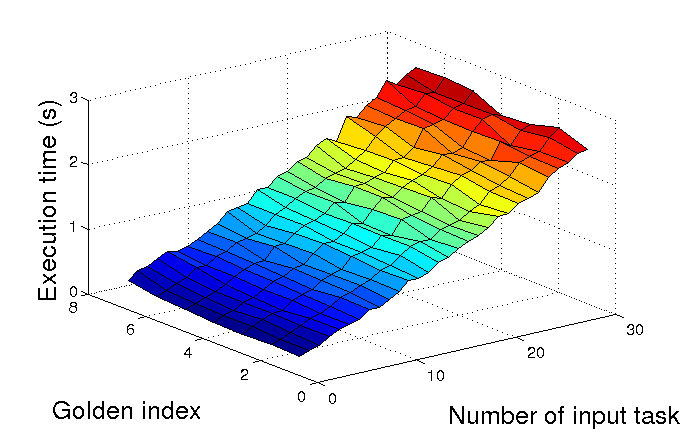
\includegraphics[width=\linewidth]{Figures/tLG_satsfix.png}
    \caption{Local-Global: execution time (satellites fixed)}\label{fig_tLG_satsfix}
  \end{minipage}  
  \begin{minipage}[b]{0.5\linewidth}
    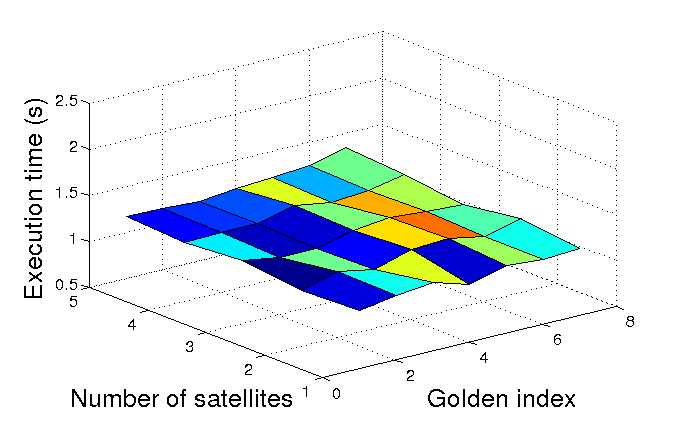
\includegraphics[width=\linewidth]{Figures/tLG_tasksfix.png}
    \caption{Local-Global: execution time (input tasks fixed)}\label{fig_tLG_tasksfix}
  \end{minipage}  
\end{figure}
\begin{figure}[h!]
  \begin{minipage}[b]{0.5\linewidth}
    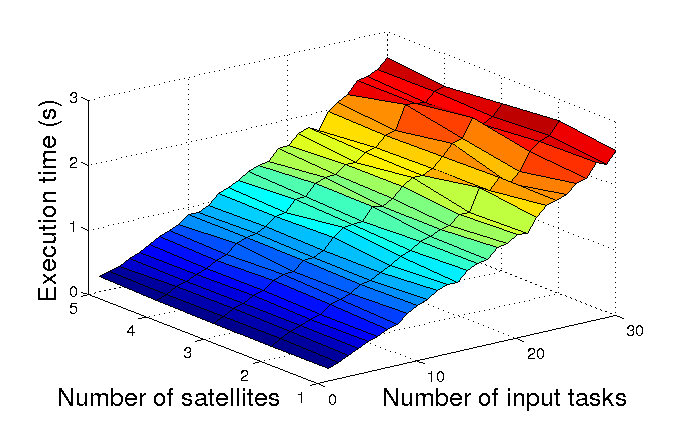
\includegraphics[width=\linewidth]{Figures/tLG_goldenfix.png}
    \caption{Local-Global: execution time (golden index fixed)}\label{fig_tLG_goldenfix}
  \end{minipage}
    \begin{minipage}[b]{0.5\linewidth}
    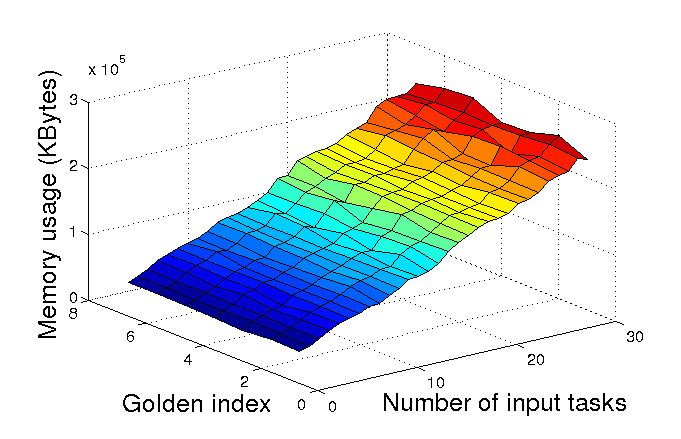
\includegraphics[width=\linewidth]{Figures/mLG_satsfix.png}
    \caption{Local-Global: memory usage (satellites fixed)}\label{fig_mLG_satsfix}
  \end{minipage}
\end{figure}
\begin{figure}[h!]
  \begin{minipage}[b]{0.5\linewidth}
    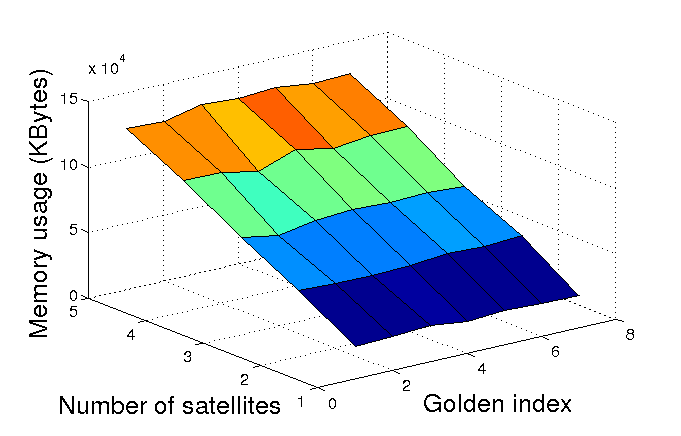
\includegraphics[width=\linewidth]{Figures/mLG_tasksfix.png}
    \caption{Local-Global: memory usage (input tasks fixed)}\label{fig_mLG_tasksfix}
  \end{minipage}  
  \begin{minipage}[b]{0.5\linewidth}
    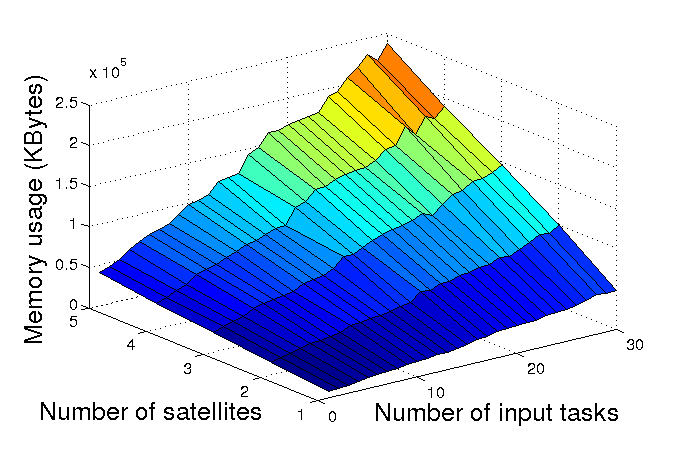
\includegraphics[width=\linewidth]{Figures/mLG_goldenfix.png}
    \caption{Local-Global: memory usage (golden index fixed)}\label{fig_mLG_goldenfix}
  \end{minipage}
  \hfill
\end{figure}

However, the improvement achieved for low values of satellites and golden index for time and memory measures is not preserved for high values, as it can be observed in figures \ref{fig_tmLG_slim}, \ref{fig_tmLG_alim}, and \ref{fig_tmLG_glim}. Nevertheless, the linear dependence from input tasks is kept.

\begin{figure}[h!]
  \begin{minipage}[b]{\linewidth}
    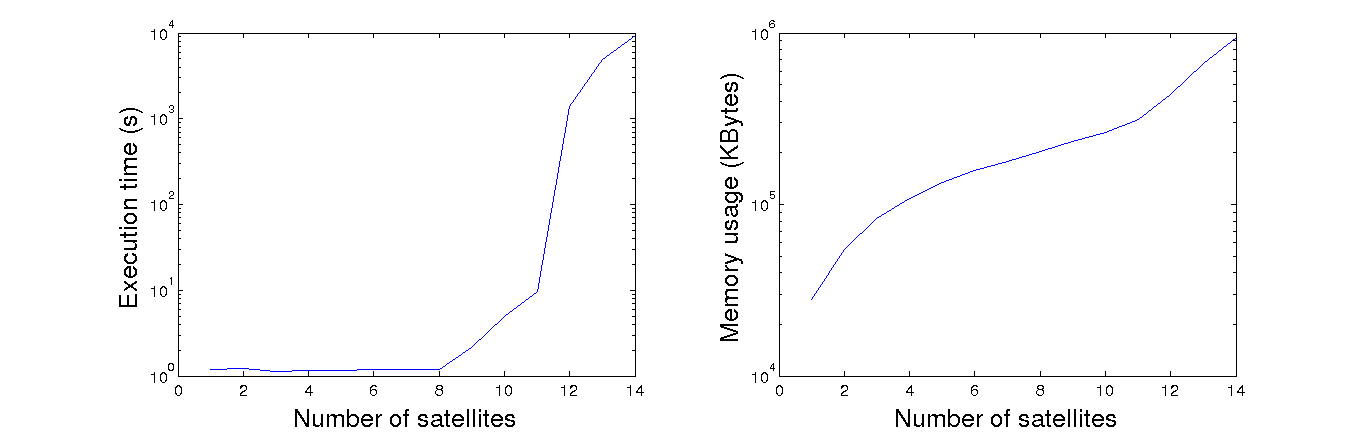
\includegraphics[width=\linewidth]{Figures/tmLG_slim.png}
    \caption{Local-Global: execution time and memory usage (varying number of satellites)}\label{fig_tmLG_slim}
  \end{minipage}
  \end{figure}
\begin{figure}[h!]
  \begin{minipage}[b]{\linewidth}
    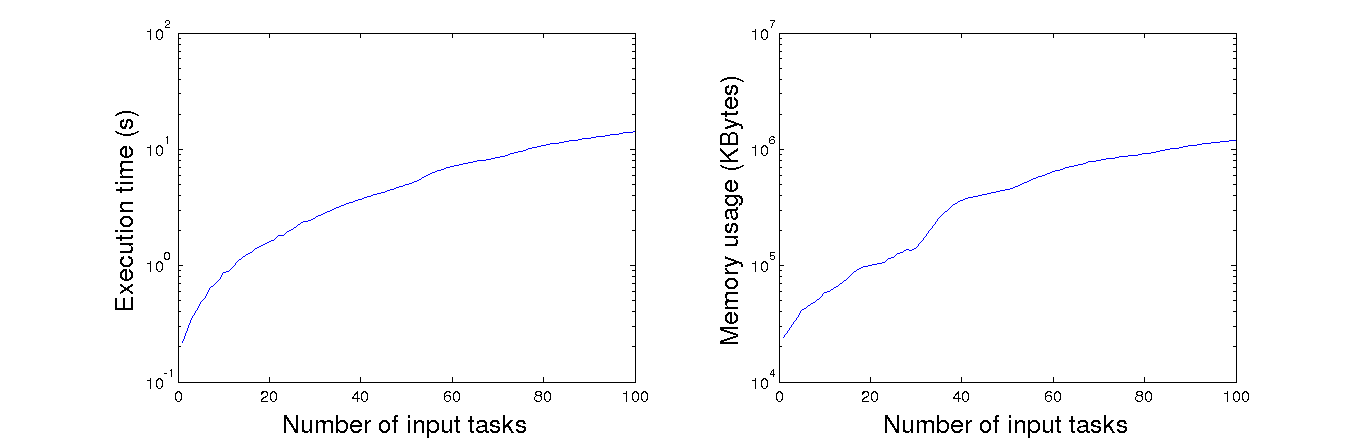
\includegraphics[width=\linewidth]{Figures/tmLG_alim.png}
    \caption{Local-Global: execution time and memory usage (varying number of input tasks)}\label{fig_tmLG_alim}
  \end{minipage}  
\end{figure}
\begin{figure}[h!]
  \begin{minipage}[b]{\linewidth}
    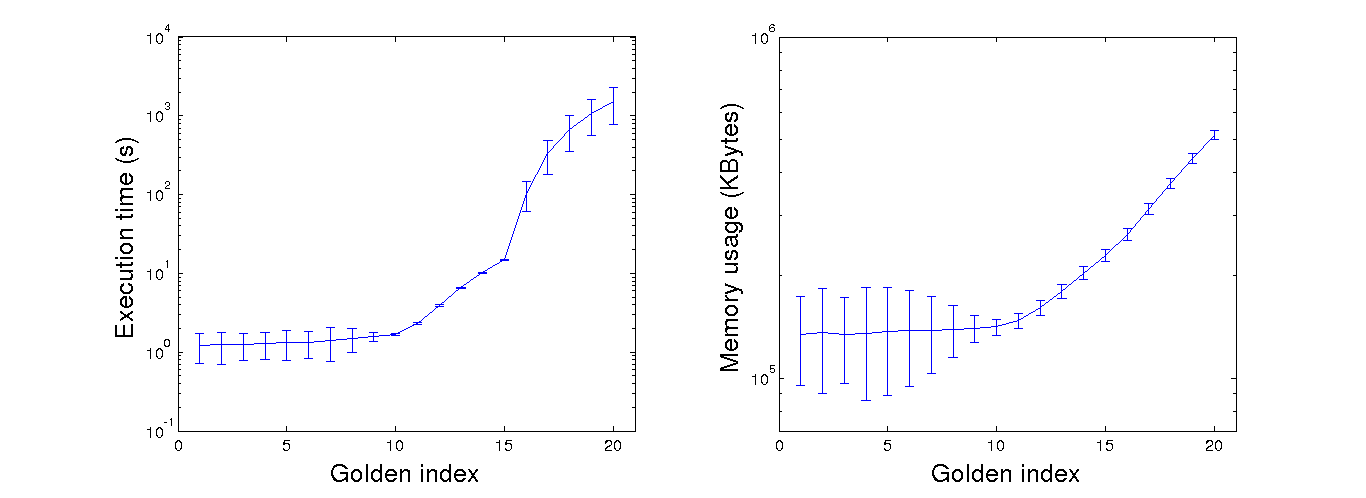
\includegraphics[width=\linewidth]{Figures/tmLG_glim.png}
    \caption{Local-Global: execution time and memory usage (varying golden index)}\label{fig_tmLG_glim}
  \end{minipage}
  \hfill
\end{figure}

Finally, the number of total scheduled tasks (i.e. the number of tasks that are present in the final schedule solution) is represented in figures \ref{fig_aLG_satsfix} (number of satellites fixed) and \ref{fig_aLG_goldenfix} (golden index fixed). Both plots are very similar and highlight an important characteristic of the Local-Global policy with the implementation carried out in this thesis: for less than 10 input tasks (in this particular benchmark) the system achieves a final schedule which schedules all the tasks available. Then, the system begins to saturate and it is not able to schedule all the input tasks. However, the ability of scheduling more tasks at high number of input tasks increases, but not at the same rate than the one of the input tasks. In Fig. \ref{fig_aLG_alim} a final constant saturation point at 80 input tasks can be observed. This behaviour can be optimized by enhancing the \emph{Local} entity so it sends better sub-solutions, as the one implemented for this Thesis still produces some suboptimal sub-solutions that affect the combining capabilities of the \emph{Global}.

\begin{figure}[h!]
  \begin{minipage}[b]{0.5\linewidth}
    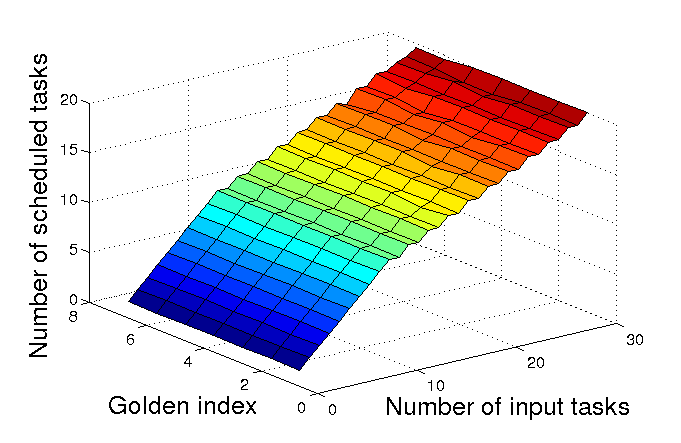
\includegraphics[width=\linewidth]{Figures/aLG_satsfix.png}
    \caption{Local-Global: scheduled tasks (satellites fixed)}\label{fig_aLG_satsfix}
  \end{minipage}   
  \begin{minipage}[b]{0.5\linewidth}
    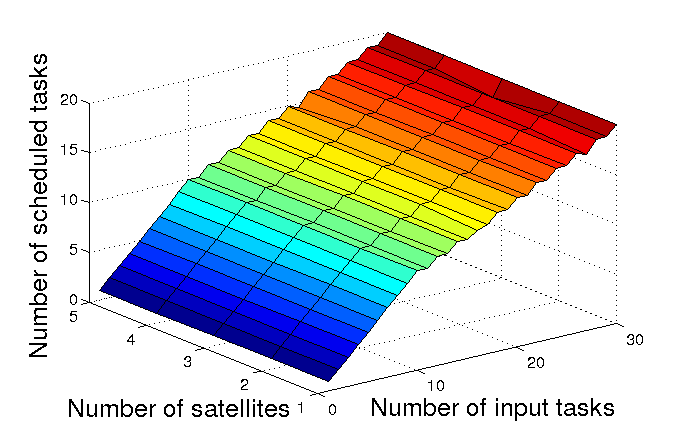
\includegraphics[width=\linewidth]{Figures/aLG_goldenfix.png}
    \caption{Local-Global: scheduled tasks (golden index fixed)}\label{fig_aLG_goldenfix}
  \end{minipage}
\end{figure}
\begin{figure}[h!]
  \begin{minipage}[b]{\linewidth}
  \centering
    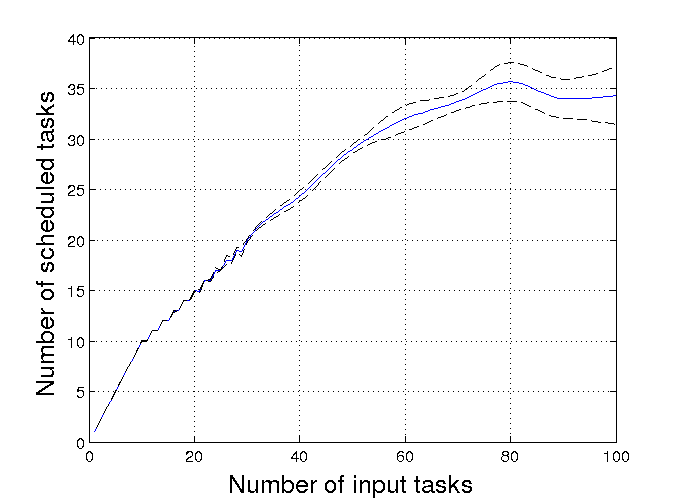
\includegraphics[width=0.6\linewidth]{Figures/aLG_alim.png}
    \caption{Local-Global: scheduled tasks for large input tasks range}\label{fig_aLG_alim}
  \centering
  \end{minipage}
  \hfill
\end{figure}

In this policy, special attention to the global combinatorial search optimizations has to be paid. In order to quickly analyse the improvement that represents to the entire policy, a performance comparison with a brute-force search has been carried out. Results are shown in Fig. \ref{fig_global_brute}, where the mitigation (in the optimized version) of exponential increase with the problem size is clearly observed.

\begin{figure}[h!]
  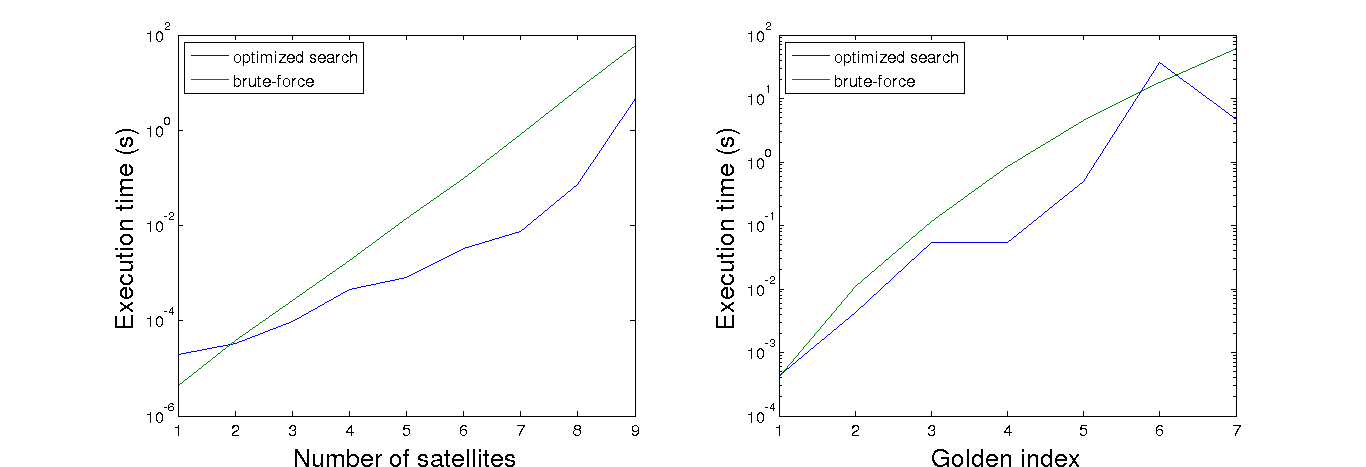
\includegraphics[width=\linewidth]{Figures/global.png}
  \caption{Global optimization: execution time comparison (combinatorial search vs. brute-force)}\label{fig_global_brute}
\end{figure}

%-----------------------------------
%	SUBSECTION 2
%-----------------------------------

\subsection{Price-based}

The price-based results are simpler, as there are only two main variables to sweep: number of satellites and number of tasks. The test results are shown in Fig. \ref{fig_tMB_sw} for time measures, in Fig. \ref{fig_mMB_sw} for memory measures and in Fig. \ref{fig_aMB_sw} for scheduled tasks number.

Regarding time and memory, a clear influence of the increase in the number of tasks is observed, while the number of satellites do not affect the final result. The results in the finally scheduled number of tasks must be highlighted: the price-based algorithm achieves to schedule almost all the input tasks for this values. However, when it is swept over the number of tasks at high values (see Fig. \ref{fig_aMB}), it can be very clearly observed that the performance decreases completely for more than 30 input tasks.

\begin{figure}[h!]
  \begin{minipage}[b]{0.5\linewidth}
    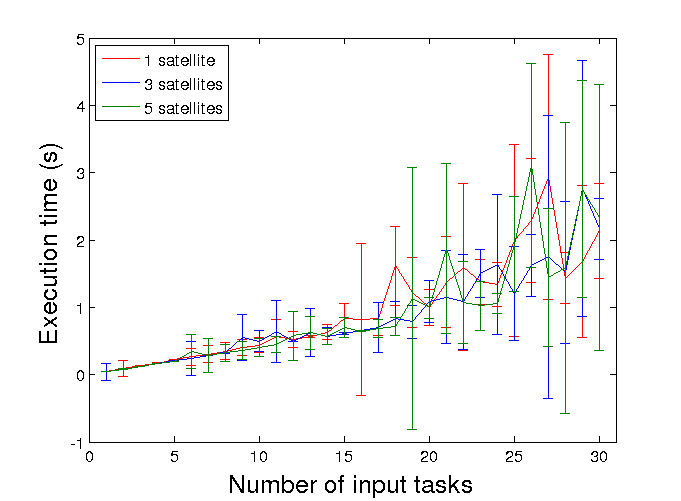
\includegraphics[width=\linewidth]{Figures/tMB_sw_2.png}
    \caption{Price-based: execution time}\label{fig_tMB_sw}
  \end{minipage} 
  \begin{minipage}[b]{0.5\linewidth}
    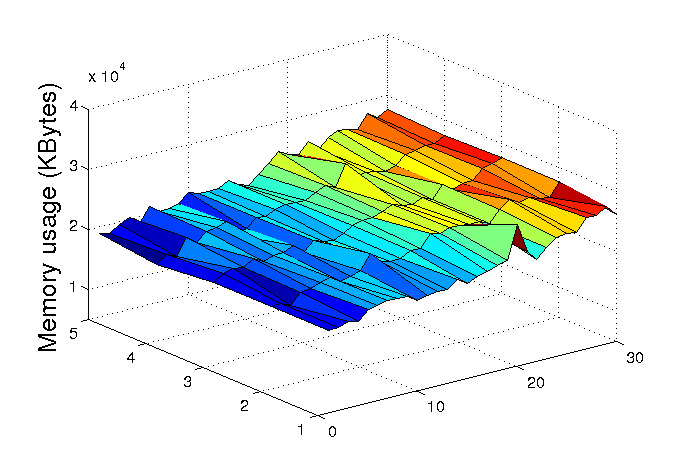
\includegraphics[width=\linewidth]{Figures/mMB_sw.png} 
    \caption{Price-based: memory usage}\label{fig_mMB_sw}
  \end{minipage} 
\end{figure}
\begin{figure}[h!]
  \begin{minipage}[b]{0.5\linewidth}
    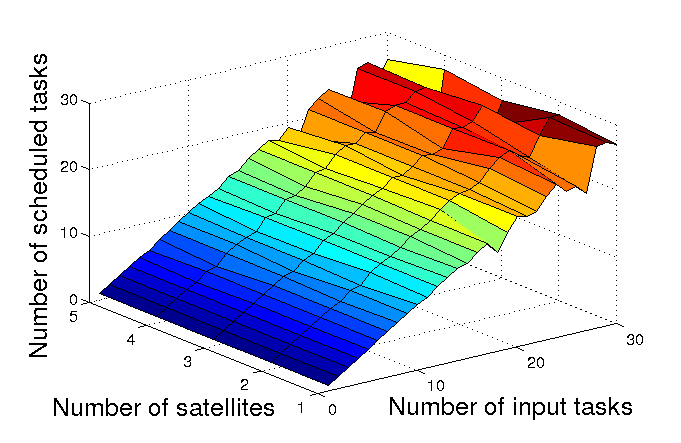
\includegraphics[width=\linewidth]{Figures/aMB_sw.png}
    \caption{Price-based: scheduled tasks}\label{fig_aMB_sw}
  \end{minipage}
    \begin{minipage}[b]{0.5\linewidth}
    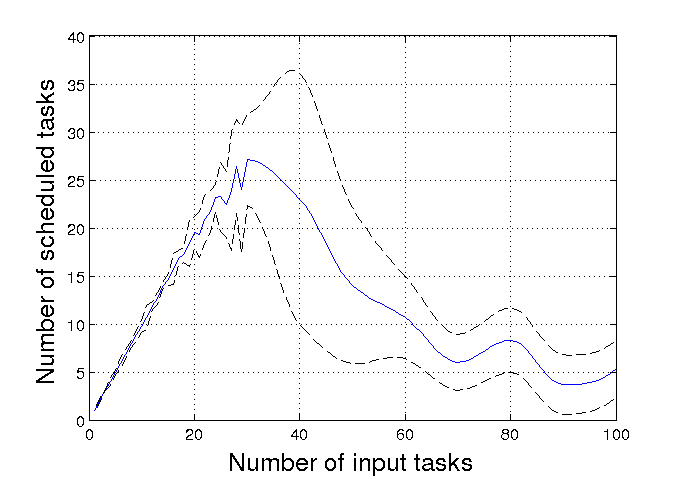
\includegraphics[width=\linewidth]{Figures/aMB.png}
    \caption{Price-based: scheduled tasks for large input tasks range}\label{fig_aMB}
  \end{minipage}
  \hfill
\end{figure}

\clearpage

%-----------------------------------
%	SUBSECTION 3
%-----------------------------------

\subsection{The comparison}

As a first concluding result, some comparison representations are shown below, highlighting now the difference in the behaviour of both schedulers that analysing separately each one can remain out of the sight.

Regarding the time spent in solving the input tests, it can be observed in Fig. \ref{fig_tLGMB} that both increasing the number of satellites or the number of tasks in the system, the price-based scheduler has lower execution times for almost all the cases. Moreover, the Local-Global policy tends to increase exponentially the resources it spends. The memory utilization behaviour is very similar to the time measures (see Fig. \ref{fig_mLGMB}).

However, it can be observed that the Local-Global policy demonstrates its strength by obtaining a constant throughput in terms of scheduled tasks (besides other parameters of the solution quality such as satellite utilization or responsiveness) when increasing the number of input tasks (see Fig. \ref{fig_aLGMB}): it achieves scheduling more tasks than the price-based scheduler for almost all the tests. The range in which the price-based performs better than the Local-Global is from 10 to 40 tasks (i.e. between the first saturation point of the Local-Global and the saturation point of the price-based).

\begin{figure}[ht]
  \begin{minipage}[b]{\linewidth}
    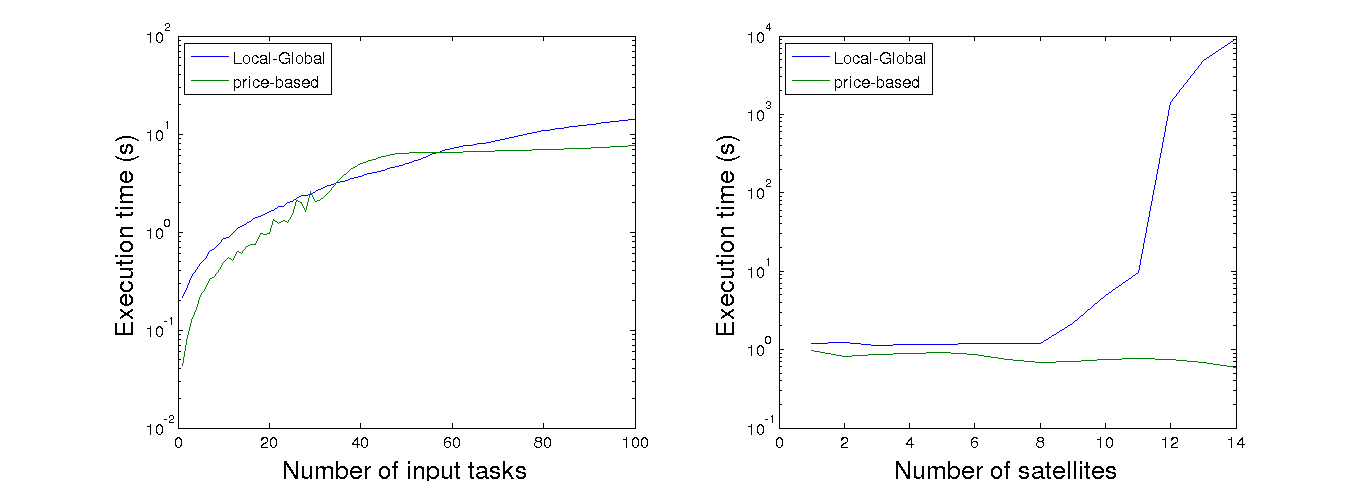
\includegraphics[width=\linewidth]{Figures/tLGMB.png}
    \caption{Local-Global vs price-based: execution time comparison}\label{fig_tLGMB}
  \end{minipage} 
\end{figure}
\begin{figure}[h!]
  \begin{minipage}[b]{\linewidth}
    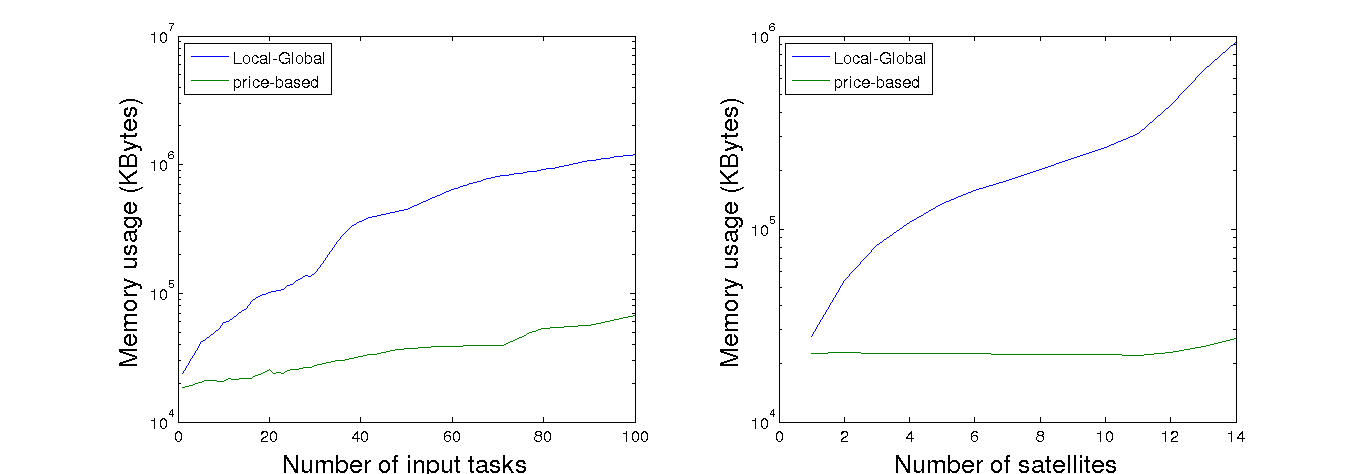
\includegraphics[width=\linewidth]{Figures/mLGMB.png} 
    \caption{Local-Global vs price-based: memory usage comparison}\label{fig_mLGMB}
  \end{minipage} 
\end{figure}
\begin{figure}[ht!]
  \begin{minipage}[t]{\linewidth}
  \centering
    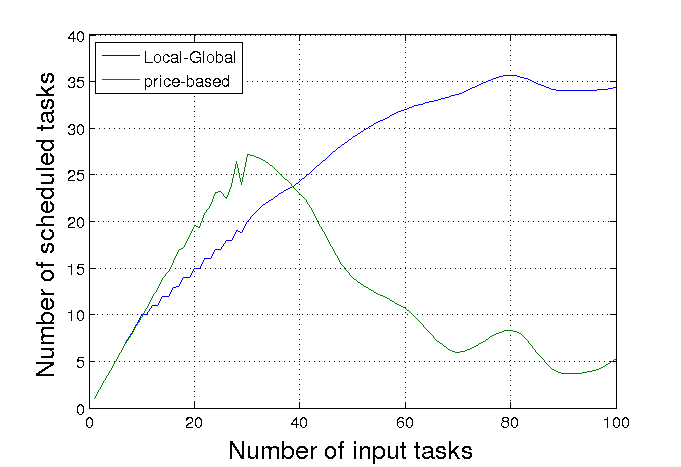
\includegraphics[width=0.6\linewidth]{Figures/aLGMB.png}
    \caption{Local-Global vs price-based: scheduled tasks comparison}\label{fig_aLGMB}
  \centering
  \end{minipage}
  \hfill
\end{figure}